\documentclass[14pt,aspectratio=169]{beamer}
\usepackage{ifxetex}
\ifxetex
  \usepackage{fontspec}
\else
  \usepackage[T1]{fontenc}
  \usepackage[utf8]{inputenc}
\fi
\usepackage[english]{babel}
\uselanguage{english}
\usetheme{simple}
\usecolortheme{whiteonblack}
\usepackage{array}
\usepackage{aurl}
\daurl{meta}{http://www.snik.eu/ontology/meta/}
\daurl{ob}{http://www.snik.eu/ontology/ob/}
\daurl{bb}{http://www.snik.eu/ontology/bb/}
\usepackage{url}
\usepackage{graphicx}
\usepackage{csquotes}
\usepackage{amssymb}
\usepackage{pifont}
\newcommand{\xmark}{\ding{55}}%
\newcolumntype{H}{>{\setbox0=\hbox\bgroup}c<{\egroup}@{}} % comment out columns
\date{2023-06-28}
\author{\texorpdfstring{Konrad Höffner\newline\url{konrad.hoeffner@uni-leipzig.de}}{Konrad Höffner}}
\title{RickView: Lightweight Standalone Knowledge Graph Browsing Powered by Rust}
\subtitle{}

\newcommand{\imageslide}[4][]
{
\begin{frame}[plain]{~~~~#2}
\vspace{0.2em}
\centering\makebox[\linewidth]{\includegraphics[width=1.13\linewidth,height=\textheight,keepaspectratio]{#3}}
\\#1
\note{#4}
\end{frame}
}

\begin{document}

\begin{frame}
\titlepage
\end{frame}

\begin{frame}{A Review of the Semantic Web Field (2021)}
\enquote{
\ldots{}what the Semantic Web field most needs, at this stage, is consolidation\ldots
For academics, there is often limited incentive to develop and maintain stable, easy-to-use software\ldots
Consolidation of sorts is already happening in industry\ldots
Technical details\ldots{} are however usually not shared, presumably to protect the own competitive edge.
}
\end{frame}

\begin{frame}{Linked Open Data Dissemination Best Practices}
\begin{itemize}
\item RDF Dump
\item SPARQL Endpoint
\item RDF Browser
\pause
\item Collaborative Editing
\item Blogs, Videos, Social Media, \ldots
\end{itemize}
\end{frame}

\begin{frame}{Dependencies}
\begin{tabular}{ll}
RDF Library		&Sophia\\% \cite{sophia}
HDT Library		&hdt-rs\\
Web Framework	&Actix Web\\
Template Engine	&TinyTemplate\\
\end{tabular}
\end{frame}

\begin{frame}{Rust---Ideal fit for the Semantic Web}
\begin{itemize}
\item fast
\item low memory
\item safe
\item modern features and tooling
\pause
\item however not that many libraries yet
\end{itemize}
\end{frame}

\imageslide{LodView}{img/lodview-screenshot.png}{}
\imageslide{RickView}{img/rickview-screenshot1.png}{}
\imageslide{RickView}{img/rickview-screenshot2.png}{}

\imageslide{LodView---Network}{img/lodview-nocache.png}{}
\imageslide{LodView---Cached}{img/lodview-cache.png}{}

\begin{frame}[plain]{RickView---Network}
\centering\makebox[\linewidth]{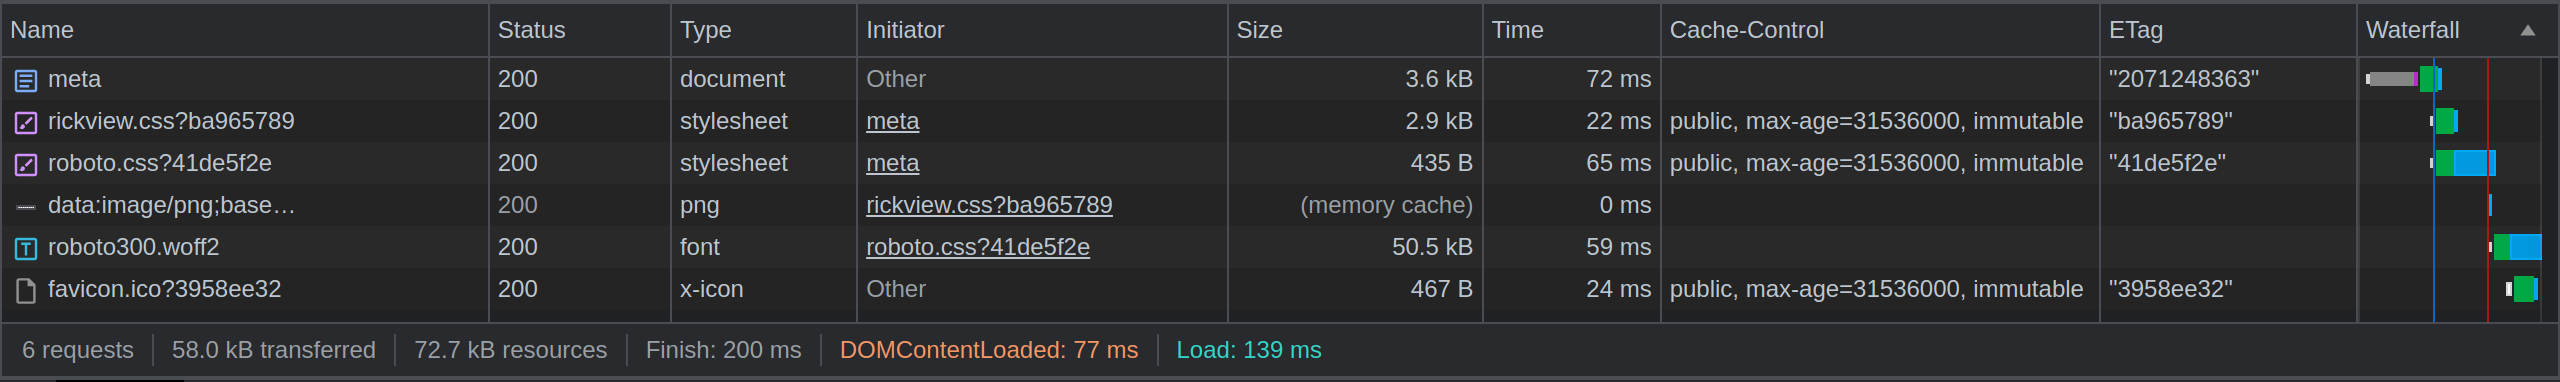
\includegraphics[width=1.13\linewidth]{img/nocache.png}}\\
\hspace{2em}
\pause
\centering\makebox[\linewidth]{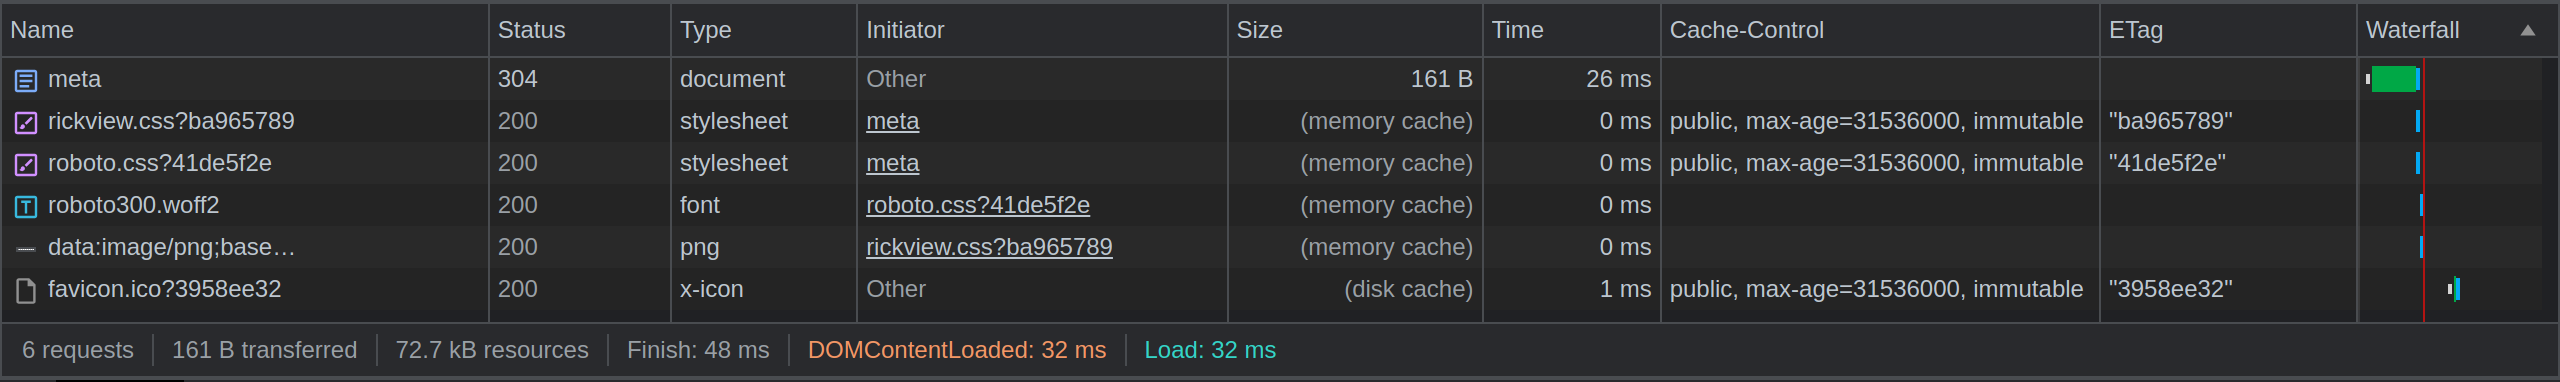
\includegraphics[width=1.13\linewidth]{img/cache.png}}
\end{frame}

\begin{frame}{Standalone}
\begin{itemize}
\item single binary $\approx 11$ MB, Alpine Docker image $\approx 18$ MB
\item includes web server
\item resources compiled into the binary
\item loads knowledge base from file or URL at start
\end{itemize}
\end{frame}

\begin{frame}{Use Case: HITO\footnote{v1.1 \url{https://hitontology.eu/ontology/}}}
\begin{itemize}
\item RickView 0.2.1: 25 MB RAM
\item LodView 1.2.1 HITO fork: 533 MB RAM + 210 MB Virtuoso
%\item Docker ulimit extension required
\end{itemize}
\end{frame}

\begin{frame}{Use Case: Linked Spending\footnote{\url{https://linkedspending.aksw.org/}}}
\begin{itemize}
\item v2014-3 file size $\approx 25$ GB N-Triples, $\approx 113$ million triples
\item original setup: extremely slow page load, crashes
\item too large for RickView, $> 32$ GB server RAM usage
\end{itemize}
\end{frame}

\begin{frame}{Use Case: Linked Spending \& HDT}
\begin{itemize}
\item Header Dictionary Triples (HDT)---compressed RDF with efficient triple pattern queries
\item Rust implementation\footnote{\url{https://github.com/konradhoeffner/hdt}} with Tim Baccaert
\item HDT Adapter for Sophia, used by RickView
\item RickView with LinkedSpending v2015 and HDT:\\$\approx 1.9$GB RAM,  $<2$ms page generation time
\end{itemize}
\end{frame}

\begin{frame}{}
%\centering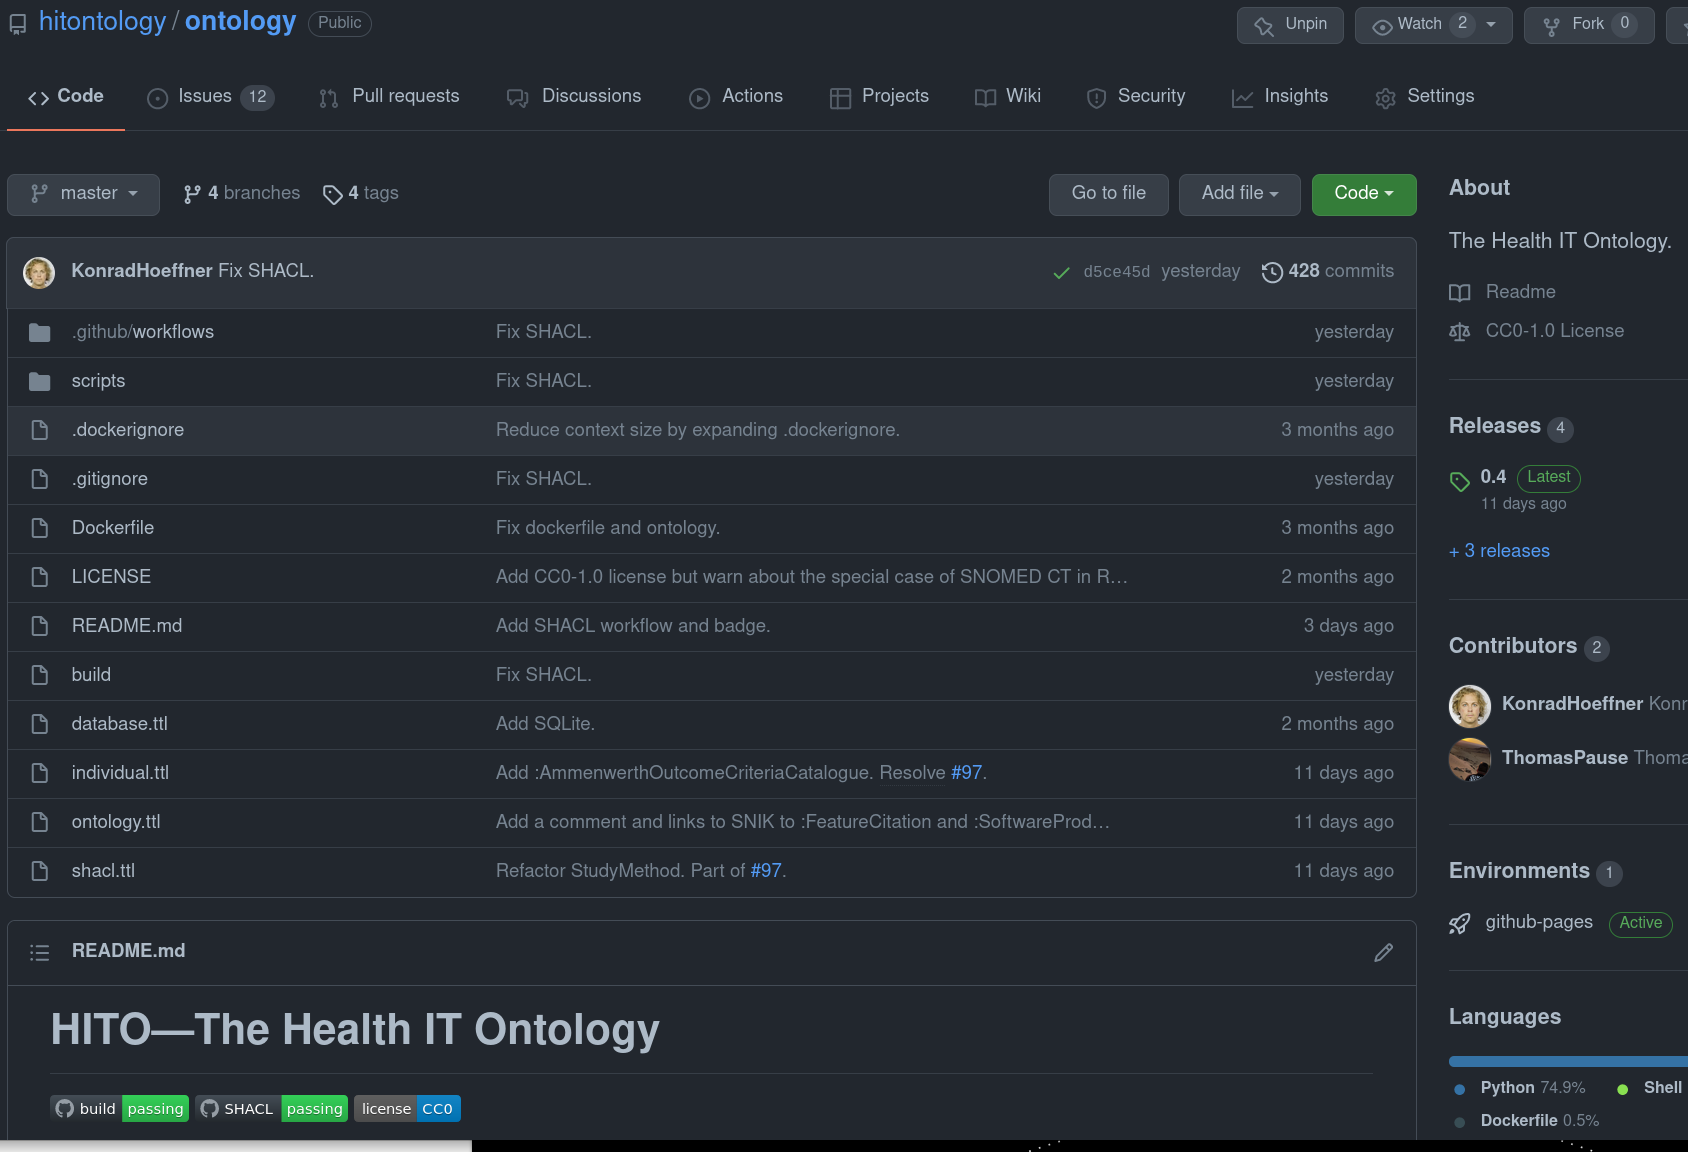
\includegraphics[width=1.05\textwidth,height=1.05\textheight,keepaspectratio]{img/github.png}
\end{frame}

\begin{frame}{}
%\centering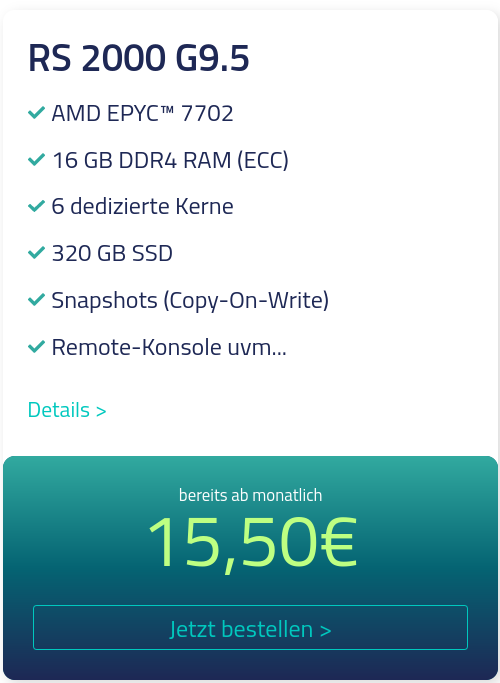
\includegraphics[width=1.05\textwidth,height=1.05\textheight,keepaspectratio]{img/netcup.png}
\end{frame}
a
\end{document}
